\documentclass{article}
\usepackage[T1]{fontenc}
\usepackage{lmodern}
\usepackage{graphicx}
\usepackage{amsmath,amssymb}
\usepackage[a4paper,margin=2cm]{geometry}
\usepackage[absolute,overlay]{textpos}
\setlength{\TPHorizModule}{1mm}
\setlength{\TPVertModule}{1mm}
\usepackage[indonesian]{babel}
\usepackage{hyperref}
\setlength{\emergencystretch}{2em}
% unit: Halaman 70

\begin{document}

% === Halaman 70 (llm) ===

\section*{Selective encryption for multimedia data}

\vspace{60mm}

Sumber: \url{https://www.researchgate.net/figure/Selective-video-encryption-and-decryption-phases_fig3_353880117}

% deskripsi: Diagram alur proses Selective Video Encryption Phase dan Selective Video Decryption Phase yang menunjukkan tahapan mulai dari Key Generation, Selection Technique, hingga menjadi bitstream terenkripsi dan proses dekripsinya kembali menjadi gambar.
% bbox normalisasi: [0.1800, 0.2260, 0.7520, 0.8980]
\begin{textblock*}{120.12mm}(37.80mm,67.12mm)
\noindent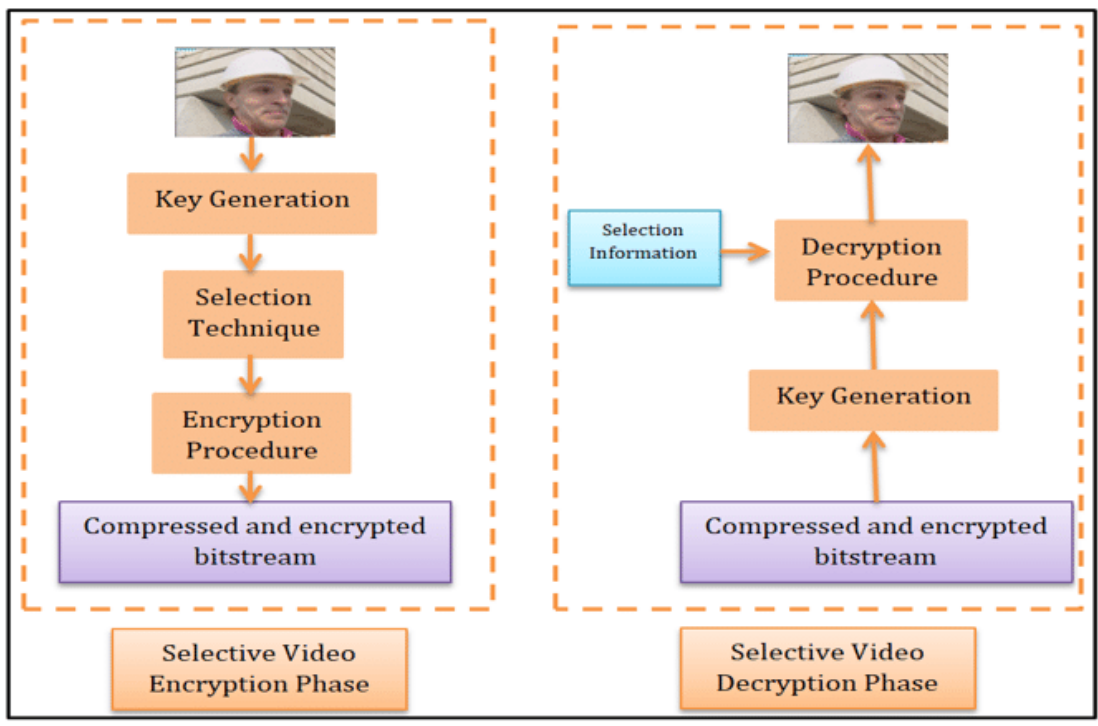
\includegraphics[width=120.12mm,height=199.58mm]{../../images/llm/page_070_img_01.png}%
\end{textblock*}

\end{document}
